\documentclass{ctexart}
\title{Algorithm Homework3}
\author{PB18111704 Zhu Enzuo}
\date{\today}
\usepackage{algorithm} %ctan.org\pkg\algorithms
\usepackage{algpseudocode}
\usepackage{amsmath}
\usepackage{tikz}
\begin{document}
\maketitle

\subsection{Prob1} 


\paragraph{a}树的形态如下:


\begin{tikzpicture}
    \node{38}
    child{
        node{\color{red}{19}}
        child{
            node{12}
            child{
                node{\color{red}{8}}
            }
            child[missing]{}
        }
        child{node{31}}
    }
    child{
        node{41}
    };
\end{tikzpicture}

\paragraph{b} 三棵红黑树依次如下:

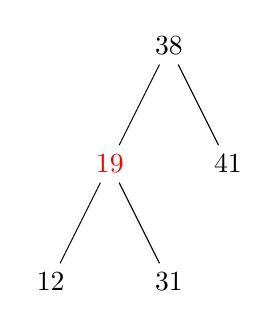
\begin{tikzpicture}
    \node{38}
    child{
        node{\color{red}{19}}
        child{
            node{12}
        }
        child{node{31}}
    }
    child{
        node{41}
    };
\end{tikzpicture}

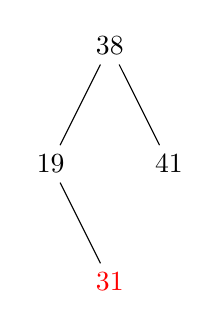
\begin{tikzpicture}
    \node{38}
    child{
        node{19}
        child[missing]{}
        child{node{\color{red}{31}}}
    }
    child{
        node{41}
    };
\end{tikzpicture}

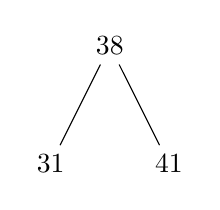
\begin{tikzpicture}
    \node{38}
    child{
        node{31}
    }
    child{
        node{41}
    };
\end{tikzpicture}

\subsection{Prob2}
\paragraph{a} Proof:我们考虑一个任取的最大覆盖点V

如果该点就是一个端点,则我们已经找到了一个端点使得命题成立。

如果该点不是一个端点,则考虑覆盖了这个点的所有区间的下界。

将下界进行排序,必然会得到一个最大的下界。而这个最大的下界的坐标必然小于该点,故覆盖选出点的所有区间的下界都小于等于该下界。

又覆盖选出点的所有区间的上界必然大于等于该点坐标,所以所有上界都大于等于选出的下界的坐标。所以所有区间
都能覆盖这个下界。故这个下界也是一个最大覆盖点。

命题得证。
\paragraph{b} 构造一颗BST保存所有上下界的坐标,其中每个节点保存如下信息:

1、权值。如果该点是一个上界则是1,如果是一个下界则是-1。

2、所有坐标小于等于该节点的点的权值之和。

对于Interval-Insert和Interval-Delete操作时都维护一次前缀和。

这样FIND-POM操作就是查询前缀和最大的点。

\subsection{Prob3}
\paragraph{a} 有问题。斐波那契堆的每一个节点的度数显然是O(logN)的。
\paragraph{b} 上界为$x.degree+2c$
\end{document}
